% Define document class
\documentclass[twocolumn]{aastex631}

\newcommand{\flatiron}{\affiliation{Center for Computational Astrophysics, Flatiron Institute, New York, NY 10010, USA}}
\newcommand{\stonybrook}{\affiliation{Department of Physics and Astronomy, Stony Brook University, Stony Brook NY 11794, USA}}
\usepackage{amsmath}
\usepackage{amssymb}
\usepackage{bm}
\usepackage{xcolor}
\usepackage{showyourwork}
\definecolor{rb4}{HTML}{27408B}
\newcommand{\kw}[1]{{\color{rb4}[KW: #1 ]}}
\newcommand{\wf}[1]{\textcolor{cyan}{WF: #1}}
\newcommand{\kb}[1]{\textcolor{pink}{#1}}
% \setlength{\floatsep}{0cm}
% \setlength{\textfloatsep}{0cm}
% \setlength{\belowcaptionskip}{-5pt}
% \setlength{\abovecaptionskip}{-5pt}
% Begin!
\begin{document}
\title{Gravitaitonal Wave Event Progenitor Synthesis}

\pacs{}

\author{Kaze W. K. Wong} 
\email{kwong@flatironinstitute.org}
\flatiron

\author{Katelyn Breivik}
\email{kbreivik@flatironinstitute.org}
\flatiron

\author{Will M. Farr}
\email{will.farr@stonybrook.edu}
\flatiron
\stonybrook


\date{\today}

\begin{abstract}
One promising way to extract information about stellar astrophysics from
gravitational wave catalogs is to compare the catalog to the outputs of stellar
population synthesis modeling with varying physical assumptions.  The parameter
space of physical assumptions in population synthesis is high-dimensional and
the choice of parameters that best represents the evolution of a binary system
may depend on an as-yet-to-be-determined way on the system's properties. Indeed,
measuring the variation of population synthesis parameter settings with binary
properties is one of the principal ways to extract information about binary
evolution from catalogs. Here we propose an inference pipeline to simultaneously
infer zero-age main sequence properties and population synthesis parameter
settings controlling modeled binary evolution from individual gravitational wave
observations of merging compact binaries.  Our pipeline can efficiently explore
the high-dimensional space of population synthesis settings and progenitor
system properties for each system in a catalog of gravitational wave
observations.  We apply our pipeline to observations in the third LIGO Virgo
Kagra Gravitational Wave Transient Catalog.  
We showcase the effectiveness of this pipeline with a detailed study
of the progenitor properties and population synthesis settings that produce
mergers like the observed GW150914.
\end{abstract}

%\maketitle

\section{Introduction}
As the detection rate of gravitation waves (GWs) from merging
double-compact-object (DCO) binaries increases with the sensitivity of the
ground-based GW detector network
\citep{Aso2013,LIGOScientificCollaboration2015,Acernese2015,Abbott2018,Buikema2020,Tse2019,Acernese2019,Akutsu2021},
we are beginning to constrain the astrophysical processes which shape the
evolution of GW progenitor populations. One of the most common ways to study
progenitor populations of GW mergers is through population synthesis simulations
of stellar populations from host of formation environments. In the case of isolated binary star evolution, merging 
double compact objects can form from massive binary stars through the
standard stable mass transfer or common envelope channels 
\citep[e.g.][]{Belczynski2002, Dominik2012, Belczynski2016, Zevin2020, Bavera2021, Broekgaarden2021, VanSon2022} 
as well as through chemically homogenous evolution \citep{Mandel2016, Marchant2016, deMink2016} 
or with population III stars \citep[e.g.][]{Belczynski2004, Kinugawa2014, Inayoshi2016, Inayoshi2017, Tanikawa2021, Tanikawa2022}.
Merging DCO binaries can also originate from a wide variety of dynamically active environments including 
triple (or higher multiple) systems \citep[e.g.][]{Antonini2017, Silsbee2017, Fragione2019, VignaGomez2021}, 
as well as young stellar clusters \citep[e.g.][]{Ziosi2014, Banerjee2017, DiCarlo2020, Chattopadhyay2022}, 
globular clusters \citep[e.g.][]{PortegiesZwart2000, OLeary2006, Downing2010, Samsing2014, Rodriguez2015, Rodriguez2016, Askar2017, Rodriguez2019}, 
nuclear star clusters \citep[][]{Miller2009, Antonini2016}, or a mix of all three \citep[e.g.][]{Mapelli2022}.
Finally, more exotic channels like active galactic nuclei which combine both gravitational and gas interactions 
\citep[e.g.][]{McKernan2018, McKernan2020, Secunda2020, Ford2021} or primordial black holes \citep[e.g.][]{Bird2016, AliHaimoud2017} 
can produce merging DCOs observable with a ground-based detector network. For a discussion of the relative rates of each 
formation environment and channels within, see \citet{Mandel2022}. 


Traditionally, population synthesis studies simulate merging DCO populations with a 
Monte-Carlo approach.  Using theoretically motivated distributions of initial parameters 
like age, metallicity, component mass, orbital separation, and eccentricity, initial 
populations are evolved with fixed astrophysical assumptions, or population synthesis 
parameter settings, to produce a synthetic catalog of DCO mergers which can be compared 
to parameterized models derived from observations. This approach contains several assumptions, 
both in the simulations and model parameterizations, which add increasing levels of 
uncertainty in population-wide comparsions of simulations and data. This compounds with the fact 
that there is no guarantee the entire population should share the same fixed hyperparameters, 
as is often assumed in most population synthesis studies.
This suggests that there could be a large (possibly infinite) family of hyper-parameter distributions 
required to compare data to simulations which span the full set of uncertain physical models.
%However, this issue is not a fundamental issue, but instead an apparent obstacle which arises from an inefficient approach to the problem.
Furthermore, each binary system could in principle come from a different formation environment and hence 
have different progenitor parameters as well as hyperparameters, which define uncertain physics associated with each environment.
Instead, it is likely advantageous to determine the posterior density in the progenitor and hyper-parameter joint space 
for each individual binary system, then perform population in analyses in that space.



%One of the most common skepticisms of population synthesis studies is that they employ simulation sets which often 
%cover a small subdomain of the entire parameter space of uncertain physics, or only vary one uncertain process per simulation
%(e.g. common envelope efficiency) while holding all others fixed to some ``default" values.
%On top of this, these values are often not calibrated to data.
While forward modelling DCO populations has been the canonical procedure to 
compare simulations to GW observations, it is also not the most efficient way 
to constrain the underlying physical processes, or ``hyperparameters", which drive the 
evolution of the population. Even with recent developments in using emulators to speed 
up the simulation process \citep[e.g.][]{Wong2021}, training the emulators 
still requires a significant amount of computation to cover a wide range of uncertainty in the hyperparemeter space.
As an example, to emulate a model with $10$ parameters, the simplest way to construct a training set of simulations is to 
run simulations on a grid which varies combinations of uncertain physics.
For $10$ uncertain physical processes, if we consider $2$ variations for each physical process 
this would still require $1024$ simulations.
Because population synthesis simulations require hundreds to thousands of cpu hours,
training an emulator which spans a high dimensional uncertainty space remains an impossibility at present.

%\kw{Reorganizing discussion related to Jeff's work such that it doesn't seem like our method is just an extension of DartBoard.}


\citet{Andrews2021} (hereafter A21) used \texttt{DartBoard} \citep{Andrews2018} 
to determine the ZAMS parameters which produce GW150914-like BBH merger based on 
posterior samples for GW150914 and a fixed 
set of hyperparameters which define assumptions for how isolated binary-star interactions proceed using 
\texttt{COSMIC}, a binary population synthesis code \citep{Breivik2020}.
However, the method was limited to a single event instead of the population.
More importantly, the method did not vary the hyperparameters while sampling the posterior density of the ZAMS parameters,
which limit its capability to be applied to understand a population of binary systems.

In this paper, we propose a method to ``backward" model each GW event to its progenitor state 
while allowing the hyper-parameters to vary across their full range of physical uncertainty
following a two-stage process.
First, we solve a root finding problem to obtain guesses that are likely to produce the 
desired system properties in the joint progenitor--hyperparameter space.
We then sample the posterior in the joint space with Markov chain Monte Carlo 
(MCMC) algorithm that is initialized using the roots found in the previous stage.
The rest of the paper is structured as follows: We detail our method in Sec. ~\ref{sec:method}.
In Sec. ~\ref{sec:result}, we show the results of applying our method to a number of real events.
We discuss the implications of this work and future direction in Sec. ~\ref{sec:discussion}.

\section{Method}
\label{sec:method}


We define the progenitor's zero age main sequence (ZAMS) properties like
mass, orbital period, and eccentricity as progenitor parameters $\bm{\theta'}$, the parameters
that control different uncertain physical prescriptions such as wind strength and common
envelope efficiency as hyperparameters $\bm{\lambda}$, and random variables
that affect certain stochastic process such as whether CO natal kick unbinds a
binary as $\bm{X}$. To avoid clutter in the following derivation, we denote all
the parameters related to mapping a particular progenitor system into a GW event
collectively as evolutionary parameters $\bm{\Theta}$, which includes
$\bm{\theta'}$, $\bm{\lambda}$, and $\bm{X}$.

Once all the parameters including a particular draw of all the random variables
represented by $\bm{X}$ are known, the population synthesis code is a
deterministic function that transforms the properties of the progenitors into
the GW parameters $\bm{\theta}$:
\begin{equation}
    \bm{\theta} = \bm{f}\left( \bm{\Theta} \right).
\end{equation}
The mapping $\bm{f}$ from $\bm{\Theta}$ to $\bm{\theta}$ can be many-to-one
due to degeneracies in the different physical processes and initial parameters  
of the GW event progenitors.
In order to draw inferences about $\bm{\Theta}$ from GW data, we
must be able to evaluate the likelihood of that data at fixed progenitor
parameters, namely
\begin{equation}
    p\left( d \mid \bm{\Theta} \right) = p\left( d \mid \bm{\theta} = \bm{f}\left( \bm{\Theta} \right) \right).
\end{equation}
The equality holds because the likelihood depends only on the gravitational waveform generated by
parameters $\bm{\theta}$ to which the progenitor parameters map onto.  In principle
this likelihood could be computed at arbitrary values of $\bm{\Theta}$ using the
same machinery that is used to estimate source parameters in GW
catalogs \citep{Veitch2015,Ashton2019,Romero-Shaw2020,GWTC-3} to develop samples
of progenitor parameters, hyperparameters, and random variables in
$\bm{\Theta}$ from a posterior density.

Since the GW likelihood function
ultimately depends only on the GW parameters $\theta$, and GWTC3 already has samples over these parameters from a posterior density 
\begin{equation}
    p\left( \bm{\theta} \mid d \right) \propto p\left( d \mid \bm{\theta} \right) \pi_\mathrm{GW} \left( \bm{\theta} \right),
\end{equation}
where $\pi_\mathrm{GW}$ is the prior density used for sampling,
we can save the computation cost associated with evaluating the GW likelihood by rewriting the posterior 
density of $\Theta$ in terms of the posterior density of $\theta$, namely

\begin{align}
    p(\Theta | d) = \frac{p(\theta(\Theta)| d) \pi(\Theta)}{\pi_\mathrm{GW}(\theta(\Theta))},
\end{align}
which we apply a kernel density estimator to the posterior samples released in GWTC3 to estimate $p(\theta(\Theta)|d)$.

Including hyperparameters and random variables %in the sampling 
drastically increases the dimensionality of the problem,
which makes the sampling process more computationally expensive to converge.
To speed up the convergence, we first solve a root-finding problem to find points that are close to the bulk of the posterior density of a GW event,
then we use those points to initialize a set of chains in the MCMC process.

%The root-finding procedure is described as follows:
For each posterior sample point in the GW-observable space,
we can find the corresponding evolutionary parameters by solving an optimization problem that minimizes 
the mean square difference between the GW event parameters and evolutionary parameters as:

\begin{align}
\mathcal{L}(\bm{\Theta},\bm{\theta}) = ||f(\bm{\Theta})-\bm{\theta}||^2.
\label{eq:loss}
\end{align}

In principle, we should only accept solutions that exactly reproduce the LVK posterior samples in the GW-observable space.
However, it is not feasible to achieve such a condition in practice, therefore we relax the condition in eq.~\ref{eq:loss} 
to a small acceptance threshold. For this study, we picked a threshold of $10^{-2}$. To make sure we find a reasonably 
complete set of progenitor parameters that corresponds to the posterior sample point, we use 1000 different initial guesses 
in solving the optimization problem. As long as the solution fulfills the acceptance criteria, the root is as valid as all 
other roots that fulfill the same acceptance criteria, \emph{regardless to its initial guess}.
This means, we have the freedom to choose the set of initial guesses however we think might benefit the optimization.

Most of the points in the evolutionary parameter space do not produce DCO mergers in a Hubble time. For systems that do not merge, 
we set the binary masses to be $0$ such that the gradient for the same systems is also $0$ and leads the root finder to get stuck on 
its first step.{\footnote{On a plateau of constant loss, the root finder performs no better than a random guess. 
Because of this, a root finder in a high dimensional space will require a significant amount of computation
to get close to a solution.}} Therefore, it is beneficial to choose initial guesses in region of the evolutionary parameter 
space that are likely to produce DCO mergers. To construct a list of initial guesses, we evolve a set of 
ZAMS parameters uniformly sampled from the initial binary parameter space, then keep the systems that 
merge within a Hubble time.

Retaining explicit control over random variables allows us to marginalize over their contribution, 
and thus allows us to focus on progenitor parameters and hyperparameters.
However, in practice most population synthesis codes (including \texttt{COSMIC} which we use in this study) 
define their random variables implicitly such that the random variables are drawn within the program instead of 
being passed as arguments. This means that the process of evolving the binary is not fully deterministic.
Thus, even if the root-finding algorithm performs perfectly, forward modelling a set of roots does not 
guarantee that the simulated population reproduces exactly the set of posterior samples due to 
randomness in the evolution of each binary. To assure that the recovered progenitor and hyperparameters 
robustly correspond to the posterior in the GW-observable space, we forward model (or "reproject") the recovered 
evolutionary parameters to the GW-observable space to check whether the reprojected posterior agrees 
with the posterior given by the LVK collaboration. 

% Validity paragraph
%\wf{What if we made this a subsection of ``methods'', and then just one sentence here about the values of the KL divergence for GW150914?}
%To check the validity of the recovered posterior over evolutionary parameters,
%it is essential to check whether it is consistent with the original posterior in
%the observable space. We reproject the recovered posterior to the observable
%space, and compare the KL divergence between the original posterior and the
%reprojected posterior. 



We use KL divergence to measure the agreement between the two posterior 
distributions as:
\begin{align}
D_{KL}(P||Q) = \int P(\bm{x}) \log(P(\bm{x})/Q(\bm{x})) dx.
\label{eq:KLdivergence}
\end{align}

\noindent A small KL divergence means the reprojected \texttt{COSMIC} posterior is similar to the original posterior in the 
observable space, and is thus a viable channel for that specific event. Otherwise, it either means \texttt{COSMIC} 
can only explain part of the posterior or cannot explain the event at all. This is completely expected behavior since 
\texttt{COSMIC}, and isolated binary evolution more generally, carries its own assumptions and is expected to 
fail in reproducing a subset of the event in GWTC3. One example of this are GW events with at least one component 
with mass above the pair instability supernova mass limit \kb{cite Farmer, and others}.
The reprojection could also be subject to stochasticity in the evolution of each binary
To account for this, we reproject the posterior multiple times with different random seeds and 
check whether the KL divergence varies significantly. A varying KL divergence means a particular GW event is subject 
to randomness in the evolution of the progenitor, and extra caution should be used when interpreting the result.


\section{Results}
\label{sec:result}
    
\begin{table*}[hbt!]
    \begin{center}
    \begin{tabular}{ l l l }
    \hline
    \hline
    Parameters &  Description & Optimization range\\
    \hline
    \hline
    Observables &\ &\  \\
    \hline
    \hline
    $m_{\rm 1, GW}$ & Primary mass of the GW event & NA \\
    $m_{\rm 2, GW}$ & Secondary mass of the GW event  & NA\\
    \hline
    \hline
    Progenitor parameters &\ &\  \\
    \hline
    \hline
    $m_{\rm 1, ZAMS}$ & Primary mass at ZAMS & $[10,150]\ M_{\odot}$\\
    $m_{\rm 2, ZAMS}$ & Secondary mass at ZAMS & $[10,150]\ M_{\odot}$\\
    $t_{\rm orb}$ & Orbital period at ZAMS & $[5,5000]$ days\\
    $e$ & Eccentricity at ZAMS & $[0,1]$\\
    $Z$ & Metallicity at ZAMS & $[10^{-4},2\times10^{-2}]$\\
    $z$ & Redshift at ZAMS & NA\\
    \hline
    \hline
    hyperparameters &\ &\ \\
    \hline
    \hline
    
    $\alpha$ & Common envelope efficiency & $[0.1,10]$\\
    $f_{\rm acc}$ & Fraction of accretion during stable mass transfer & $[0,1]$\\
    $q_{\rm crit,3}$ & Critical mass ratio on the Hertzsprung Gap & $[0.1,10]$\\
    $\sigma$ & Root mean square of Maxwellian natal kick distribution& $[10,300]\ {\rm km/s}$\\


    \hline
    \hline
    \end{tabular}
    \caption{A list of parameters we used in this study.}
    \label{tab:parameters}
    \end{center}
\end{table*}

We apply the method described in section \ref{sec:method} to the first GW event GW150914.
The parameters involved in the analysis and the range we allow for the inference are tabulated in table \ref{tab:parameters}.
The spin of BHs formed in isolated binaries depends strongly on the angular 
momentum transport in massive stars which is still highly uncertain \kb{(see however Bavera+, fuller+)},
therefore we only consider the two component masses in the observable space in the both the 
root-finding stage and the MCMC stage. For progenitor parameters, we characterize each guess with 
five parameters: the two component masses $M_{\rm 1,ZAMS}$ and $M_{\rm 2,ZAMS}$, the orbital period $t_{\rm orb}$, 
the eccentricity $e$, the metallicity $Z$ at ZAMS. Note that the progenitor formation redshift is not 
obtained through the root-finding process because the formation redshift does not intrinsically affect 
the evolution of the binary. Instead, we compute the time it takes for the binary to evolve from 
formation to the merger and add this time back to the lookback time when a GW event is observed and limit the total 
time to merger to be less than $13.7\,\rm{Gyr}$.
Using the total lookback time, we can compute the redshift of the binary at ZAMS formation following the 
Planck 2018 cosmological model \citep{Planck2018}.
The main benefit of post-processing the redshift in this way is that we do not rely on a particular assumption
of star formation rate (SFR) distribution when we solve for the posterior distribution in redshift.
This means we can put the prior on formation redshift (or in general, metallicity-redshfit distribution) in
by reweighting the posterior distribution according to a particular SFR model,
and therefore do not have to rerun the inference everytime we change the SFR model. This is especially helpful
since SFR models are still highly uncertain but strongly impact the local merger rates of BBHs \citep{Broekgaarden2021}.
For hyperparameters, we choose parameters that affect 
binary evolution in \texttt{COSMIC} mostly significantly for massive stars, including the common envelope 
efficiency $\alpha$, the fraction of mass accreted onto the accretor during stable mass transfer $f_{\rm acc}$, 
the critical mass ratio which determines whether Roche-overflow mass transfer 
proceeds stably or produces a common envelope when the donor star is on the Hertzsprung gap 
$q_{\rm crit,3}$, and the root-mean-square of the Maxwellian distribution
employed for CO natal kicks, $\sigma$. 

We show a portion of the joint posterior of the progenitor parameters and
hyperparameters of GW150914 in figure \ref{fig:GW150914_posterior}. Each panel
is colored based on the comparison between progenitor parameters (blue),
hyperparameters (orange), or a mix of the two (green). We find that the choice
for $\sigma$ does not affect the formation of GW150914-like BBHs. This is not
unexpected since we use the \citet{Fryer2012} delayed model which reduces the
natal kick strength at BH formation based on the amount of fallback onto the
proto-CO. In the case of GW150914-like BBHs, the BH progenitors are massive
enough that the fallback reduces the natal kick to zero. Because of this we do
not include $\sigma$ in Figure~\ref{fig:GW150914_posterior}. Similarly, we do
not include the ZAMS orbital period and eccentricity, which are correlated with
one another, but not strongly with the other progenitor parameters or
hyperparameters. We find strong correlations between the ZAMS masses, as well as
strong correlations between $M_{2,\rm{ZAMS}}$ and $f_{\rm{acc}}$, and
$f_{\rm{acc}}$ and $\alpha$. We show scatter plots of each of these combinations
in the upper-right inset of the figure.

The correlations between the ZAMS masses are similar to those found by A21 with
the majority of the population preferring primary and secondary masses between
$60$--$90\,M_{\odot}$. However, we also find some ZAMS masses which extend up to
$150\,M_{\odot}$ which is the limit imposed by our assumptions. We explore the
formation scenarios which lead to successful GW150914-like mergers and those
which fail to produce GW150914-like mergers below in
Figure~\ref{fig:compare_fixed_variable}.

The correlations between $M_{2,\rm{ZAMS}}$ and $f_{\rm acc}$ illustrate the
variety of ways which GW150914-like mergers can be produced. For binaries with
$M_{2,\rm{ZAMS}} < 70\,M_{\odot}$, we find that accretion efficiencies of
$f_{\rm acc} > 0.5$ are preferred. One reason for this is based on the
requirement that the total mass in the binary must remain above the total mass
of GW150914 and strongly non-conservative mass transfer (i.e. $f_{\rm acc} <
0.5$) reduces the total mass of the system. A compounding factor is that as mass
leaves the binary due to non-conservative mass transfer, the evolution of the
binary's orbit is less dramatic and leads to wider binaries on average and thus
fewer mergers in a Hubble time. For binaries with $M_{2,\rm{ZAMS}} \sim
80\,M_{\odot}$, $f_{\rm acc}$ is less constrained. This is because of a
preference for these secondaries to also have primary masses near $
80\,M_{\odot}$ and thus enter a double-core common envelope evolution in which
both stars' envelopes are ejected, leaving behind two stripped helium cores in a
tight orbit. In this case, $f_{\rm acc}$ does not affect the binary evolution
and is thus unconstrained. This effect can also be seen in the ZAMS mass and
$q_{\rm crit 3}$ panels for masses near $80\,M_{\odot}$ because double-core
common-envelope evolution is triggered in \texttt{COSMIC} when the radii of the
two stars touch due to the rapid expansion of the primary star upon helium
ignition. In this case, the choice for Roche-overflow mass transfer to proceed
stably (as prescribed by $f_{\rm{acc}}$) or unstably (as prescribed by $\alpha$)
using $q_{\rm crit, 3}$ is totally irrelevant, and thus unconstrained. Finally,
for binaries with $M_{2,\rm{ZAMS}} > 80$, we find that $f_{\rm acc}$ is
correlated to decrease with increasing mass. This is due to limits on the total
mass which must be ejected from the binary to produce BH masses that match
GW150914, the reverse situation to $M_{2,\rm{ZAMS}} < 70 \, M_\odot$. Binaries
with both component masses near $150\,M_{\odot}$ must either go through a common
envelope evolution (in which case $f_{\rm acc}$ is unconstrained), or very
non-conservative mass transfer (where $f_{\rm acc}$) is low, to produce BBHs
with the proper mass.

Finally, we find that $\alpha$ and $f_{\rm acc}$ are largely uncorrelated,
though there exist independent trends in each hyper parameter. This is not
totally unexpected since the physical processes which are described by each
hyperparameter, i.e. stable Roche-lobe overflow and common envelope evolution
are two independent channels. Generally, we find that GW150914-like BBHs tend to
prefer larger accretion efficiencies and have common envelope ejection
efficiencies peaking near $\alpha=1$. One shortcoming of our method
implementation is the application of a single hyper parameter for
$f_{\mathrm{acc}}$ and $\alpha$ for each binary, while both the primary and the
secondary star could in principle be defined by their own hyperparameters that
prescribe the outcomes for when each star fills it's Roche lobe. We reserve full
treatment of this for future work but note that this improvement could reveal
correlations between hyperparameters that are not present in our current
analysis.


\begin{figure*}[h]
    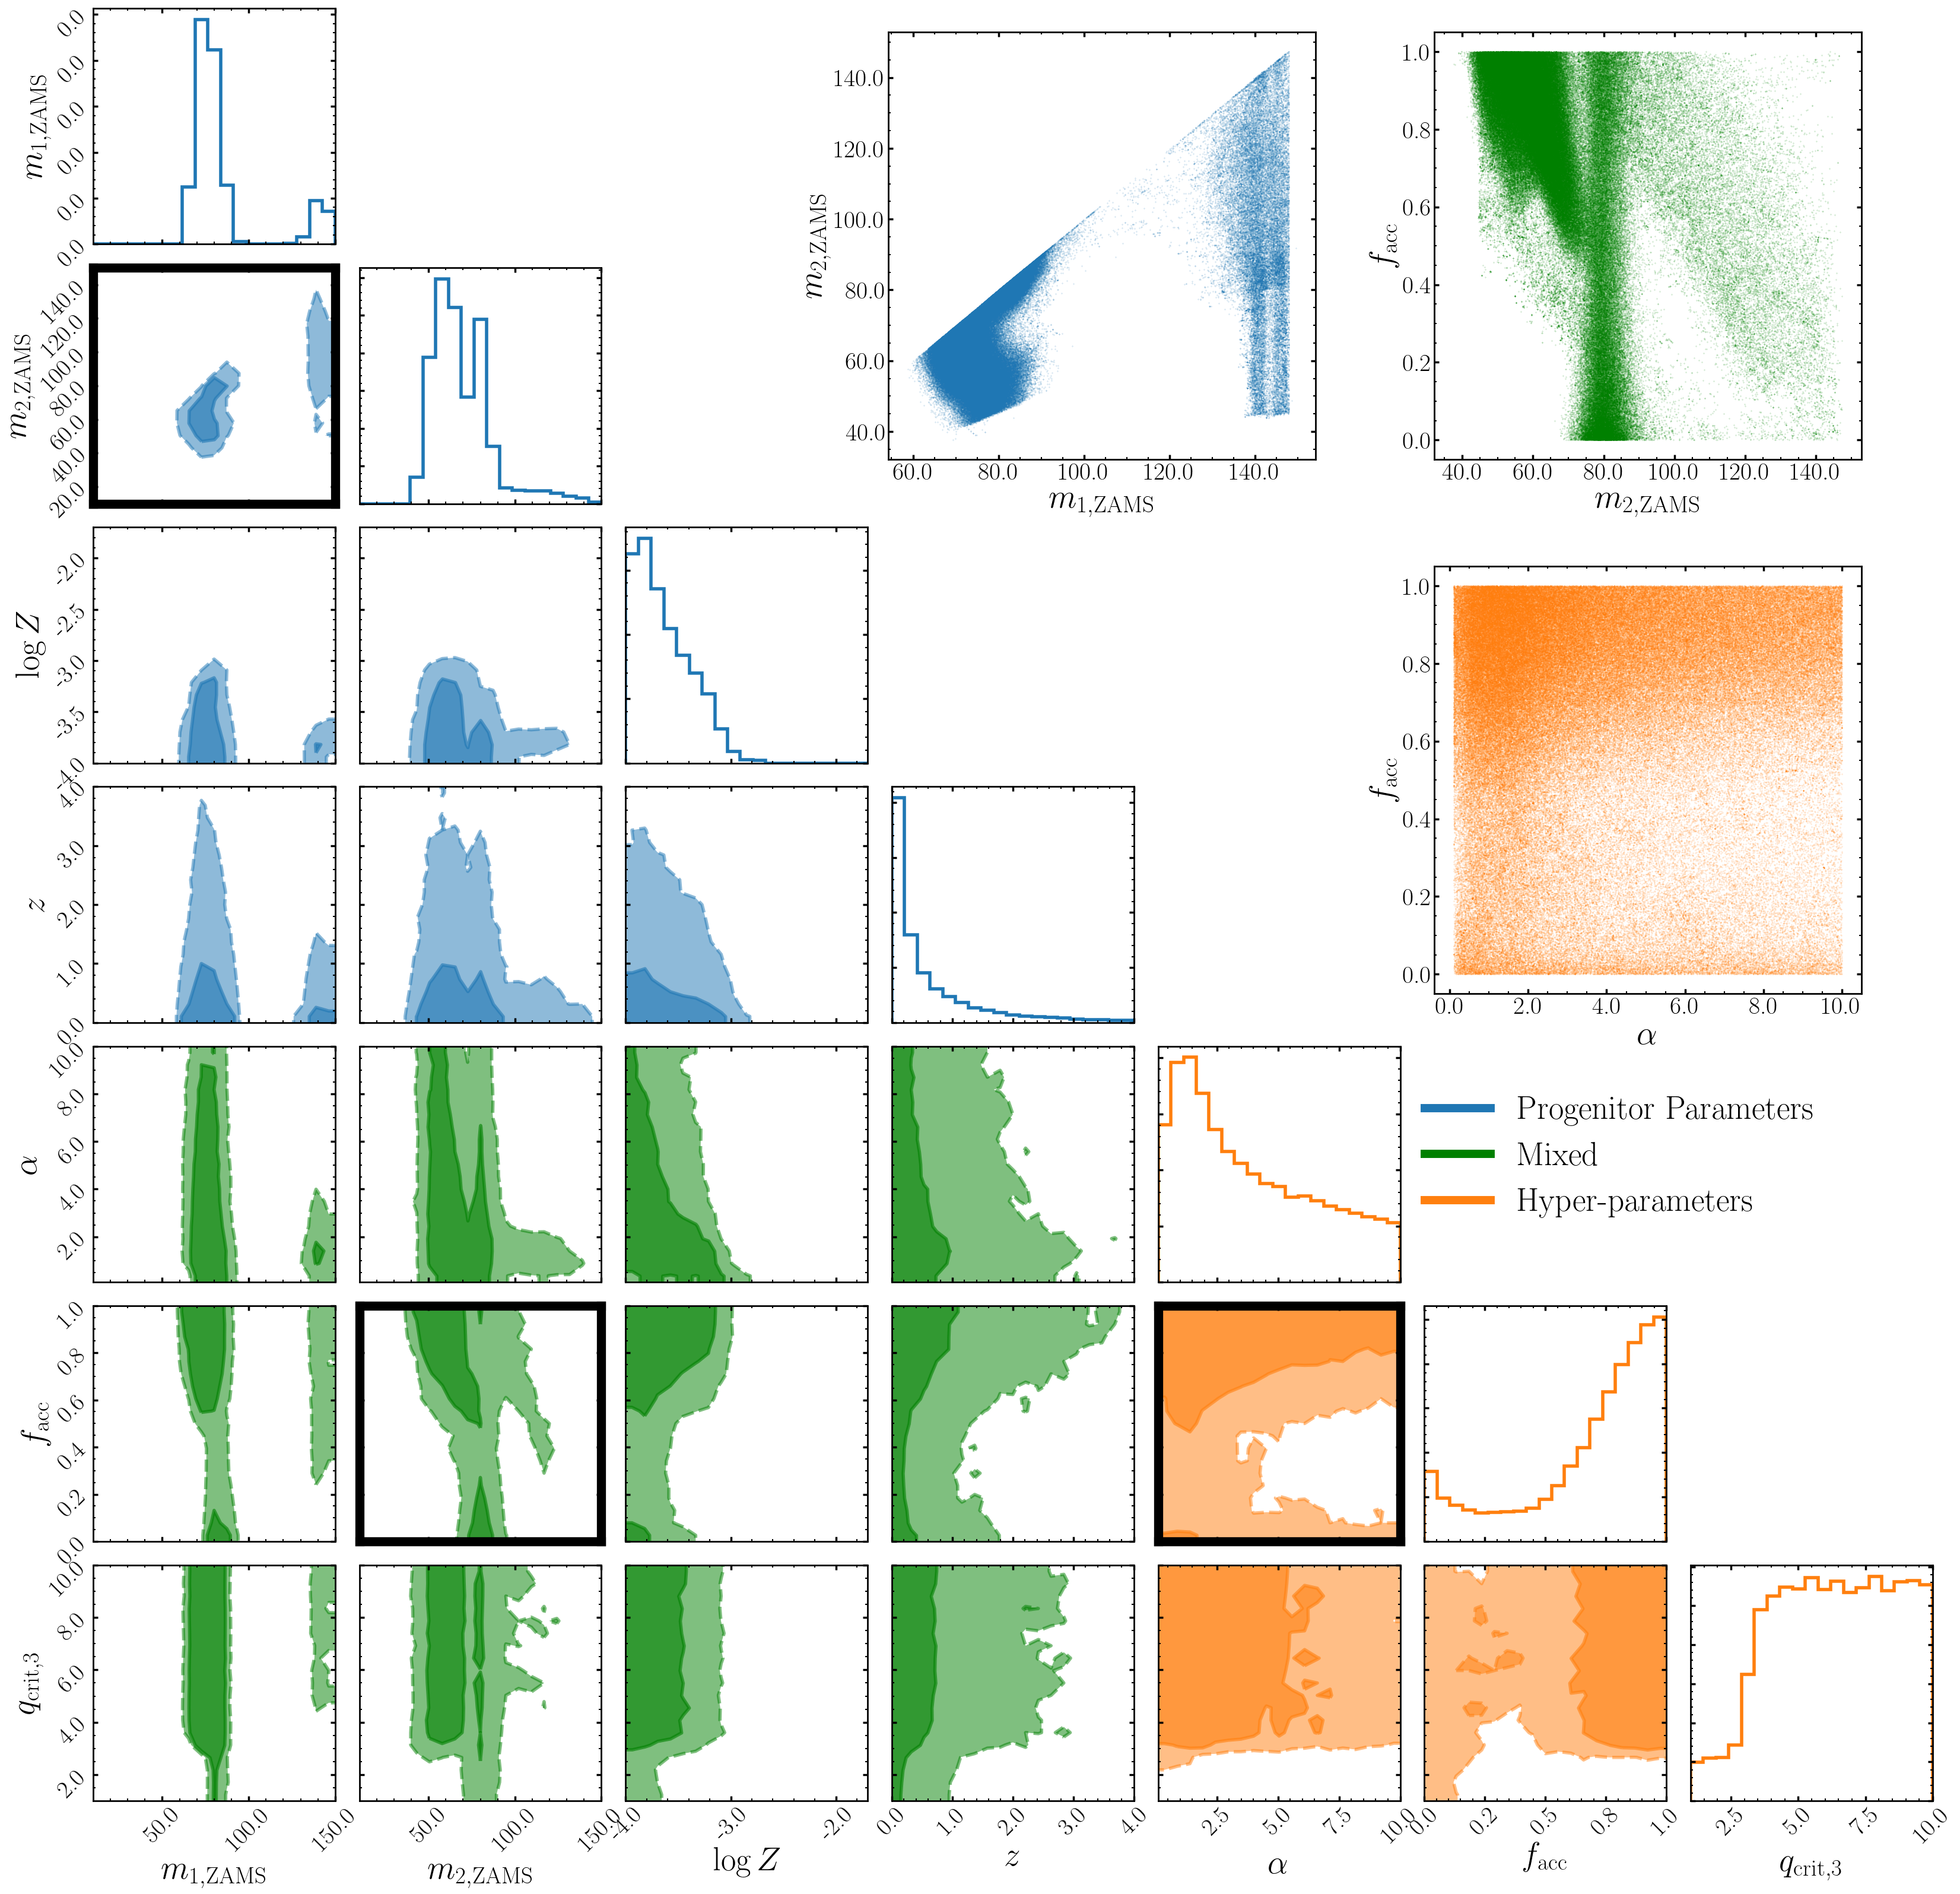
\includegraphics[width=\textwidth]{figures/GW150914_corner_zoomed_lowres.png}
    \caption{The posterior for GW150914 in both the progenitor parameter space and hyper-parameter space.
    $M_1$ and $M_2$ are the progenitors' masses. $\log{Z}$ is log metallicity at ZAMS.
    $z$ is the redshift at ZAMS. 
    $\alpha$ is the common envelope efficiency.
    $f_{\rm acc}$ is the fraction of mass accreted during stable mass transfer.
    $q_{\rm crit 3}$ is the critical mass ratio on the Hertzsprung Gap,
    Note that the redshift is not fitted during the root finding process or the MCMC process.
    Once we have find the evolutionary parameters, we add the delay time to the lookback time of the observed posterior sample,
    then from the total lookback time we can compute the redshift at ZAMS.
    We highlight three panels in the corner plots to show the fine structure of the set of posterior samples in the evolutionary parameter space.
    We also color the posterior in a particular panel according to the type of parameters involved in the corner.
    Blue denotes panels that include only progenitor parameters,
    green denotes panels that include a mix of progenitor and hyperparameters,
    and orange denotes panels that include only hyperparameters.
    }
    \label{fig:GW150914_posterior}
    \script{figure1_cornerPlot.py}
\end{figure*}

Once we obtain a set of binaries which successfully map the ZAMS parameters and
hyperparameters to BBH merger masses, we re-evolve the set of ZAMS parameters
with the same physical assumptions as A21, but vary the common envelope
efficiency to explore how keeping a fixed model which only varies one
hyper-parameter contrasts to our results.
Figure~\ref{fig:compare_fixed_variable} shows the distribution of ZAMS masses
for three models (first through third columns), each with a different $\alpha$
but the same hyper-parameters as A21, as well as the results of our sampling
which allows our hyper-parameters to vary (fourth column). We find that holding
the accretion efficiency, $f_{\rm{acc}}$, and common envelope ejection
efficiency, $\alpha$, to fixed values greatly reduces the ZAMS parameter space
that produces GW150914-like mergers. In contrast, by allowing the
hyper-parameters to fully span the model uncertainty, we find that there are
distinct ZAMS parameters which produce GW150914-like mergers.  

Because we can explore the full evolutionary parameter space, we can also
determine that there are ZAMS parameters which fail to produce GW150914-like
mergers \emph{regardless of our hyper-parameter choice.} For primary ZAMS masses
between $\sim95-135\,M_{\odot}$ and secondary ZAMS masses between
$\sim50-95\,M_{\odot}$, we find that there is no combination of accretion
efficiency and common envelope ejection efficiency which produces merging BBHs
that have masses consistent with GW150914's posteriors. In this region, if BBHs
with masses consistent with GW150914's masses are produced through a combination
of $\alpha$ and $f_{\rm{acc}}$, they do not merge in a Hubble time. Conversely,
in the region of the fourth column of Figure~\ref{fig:compare_fixed_variable}
which does produce GW150914-like mergers, the combination of $\alpha$,
$f_{\rm{acc}}$, and the ZAMS masses and orbital separations balance to produce
BHs with the correct masses that merge within a Hubble time.


\begin{figure*}
    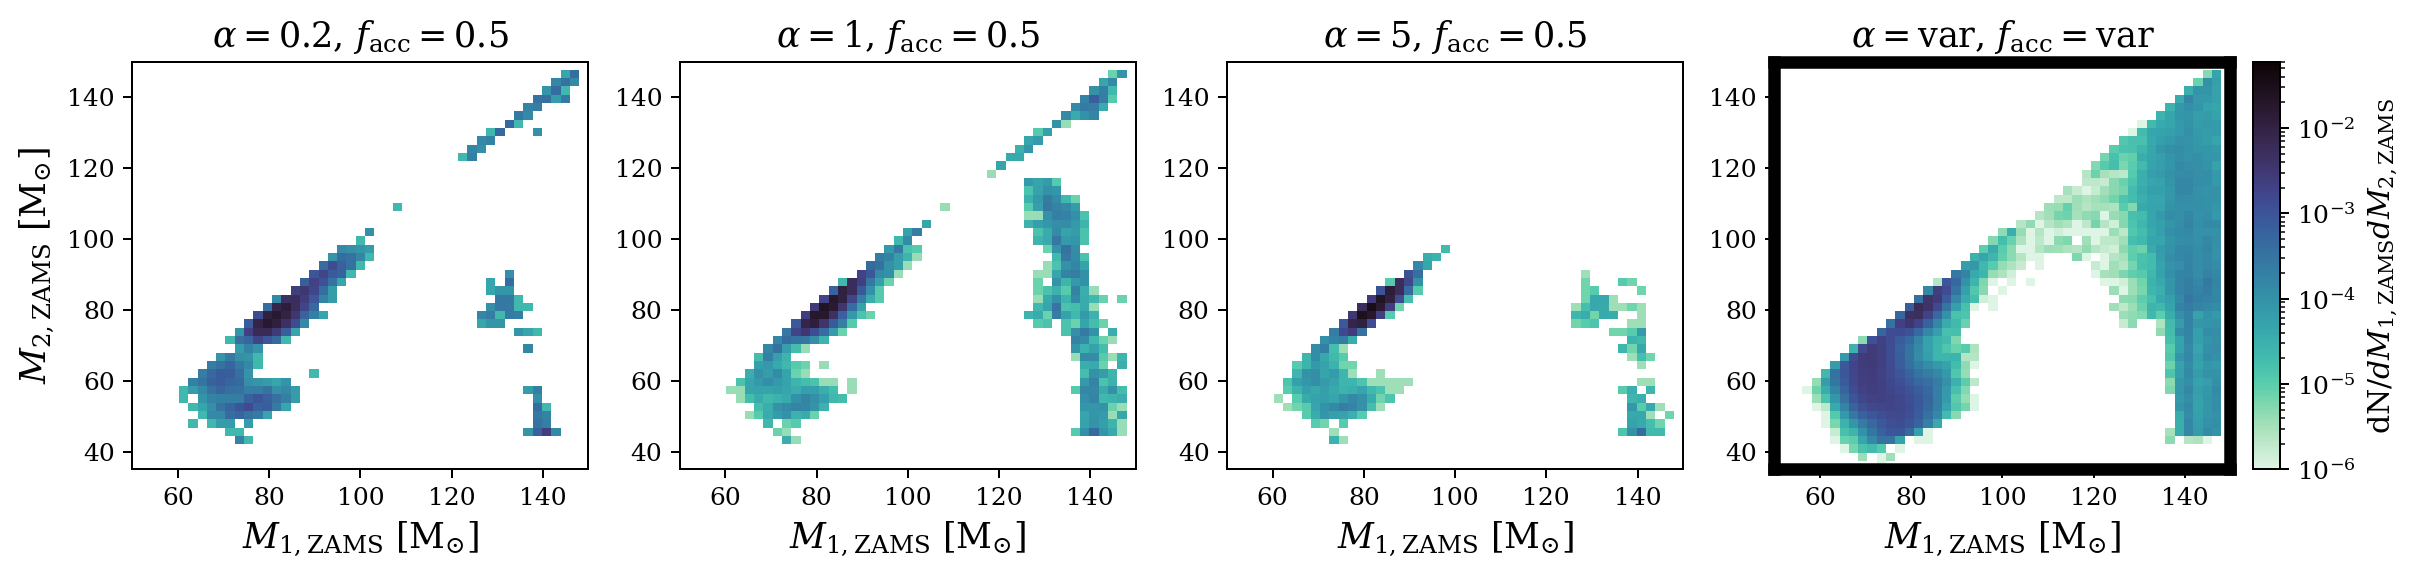
\includegraphics[width=0.98\textwidth]{figures/compare_fixed_variable.png}
    \caption{Comparison of ZAMS masses for binaries which produce GW150914-like mergers for three variations of $\alpha$
     with fixed set of parameter assumptions matching those of A22 (first three columns) and for binaries which produce 
     GW150914-like mergers when $\alpha$, $f_{\mathrm{acc}}$, and $q_{c,3}$ are allowed to vary, (fourth column).}
    \label{fig:compare_fixed_variable}
    \script{figure2_varyAlphaFacc.py}
\end{figure*}

It is interesting to re-project the posterior over progenitor ($\bm{\theta}'$)
and hyperparameters ($\bm{\lambda}$) using fresh random variables ($\bm{X}$) to
the observable space of GW parameters ($\bm{\theta}$).  Agreement between the
observed parameters and the re-projected parameters indicates good exploration
of the random variable space and lack of sensitivity to the details of these
random parameters.  Figure \ref{fig:GW150914_reprojection} shows good agreement
between the re-projected root-finding outputs as well as the re-projected MCMC
draws for our analysis of GW150914.  Unlike \citet{Andrews2021}, we find there
are no regions of observable space inaccessible to our evolutionary models; this
difference arises because we allow the evolutionary hyperparameters
$\bm{\lambda}$ to vary.

\begin{figure}
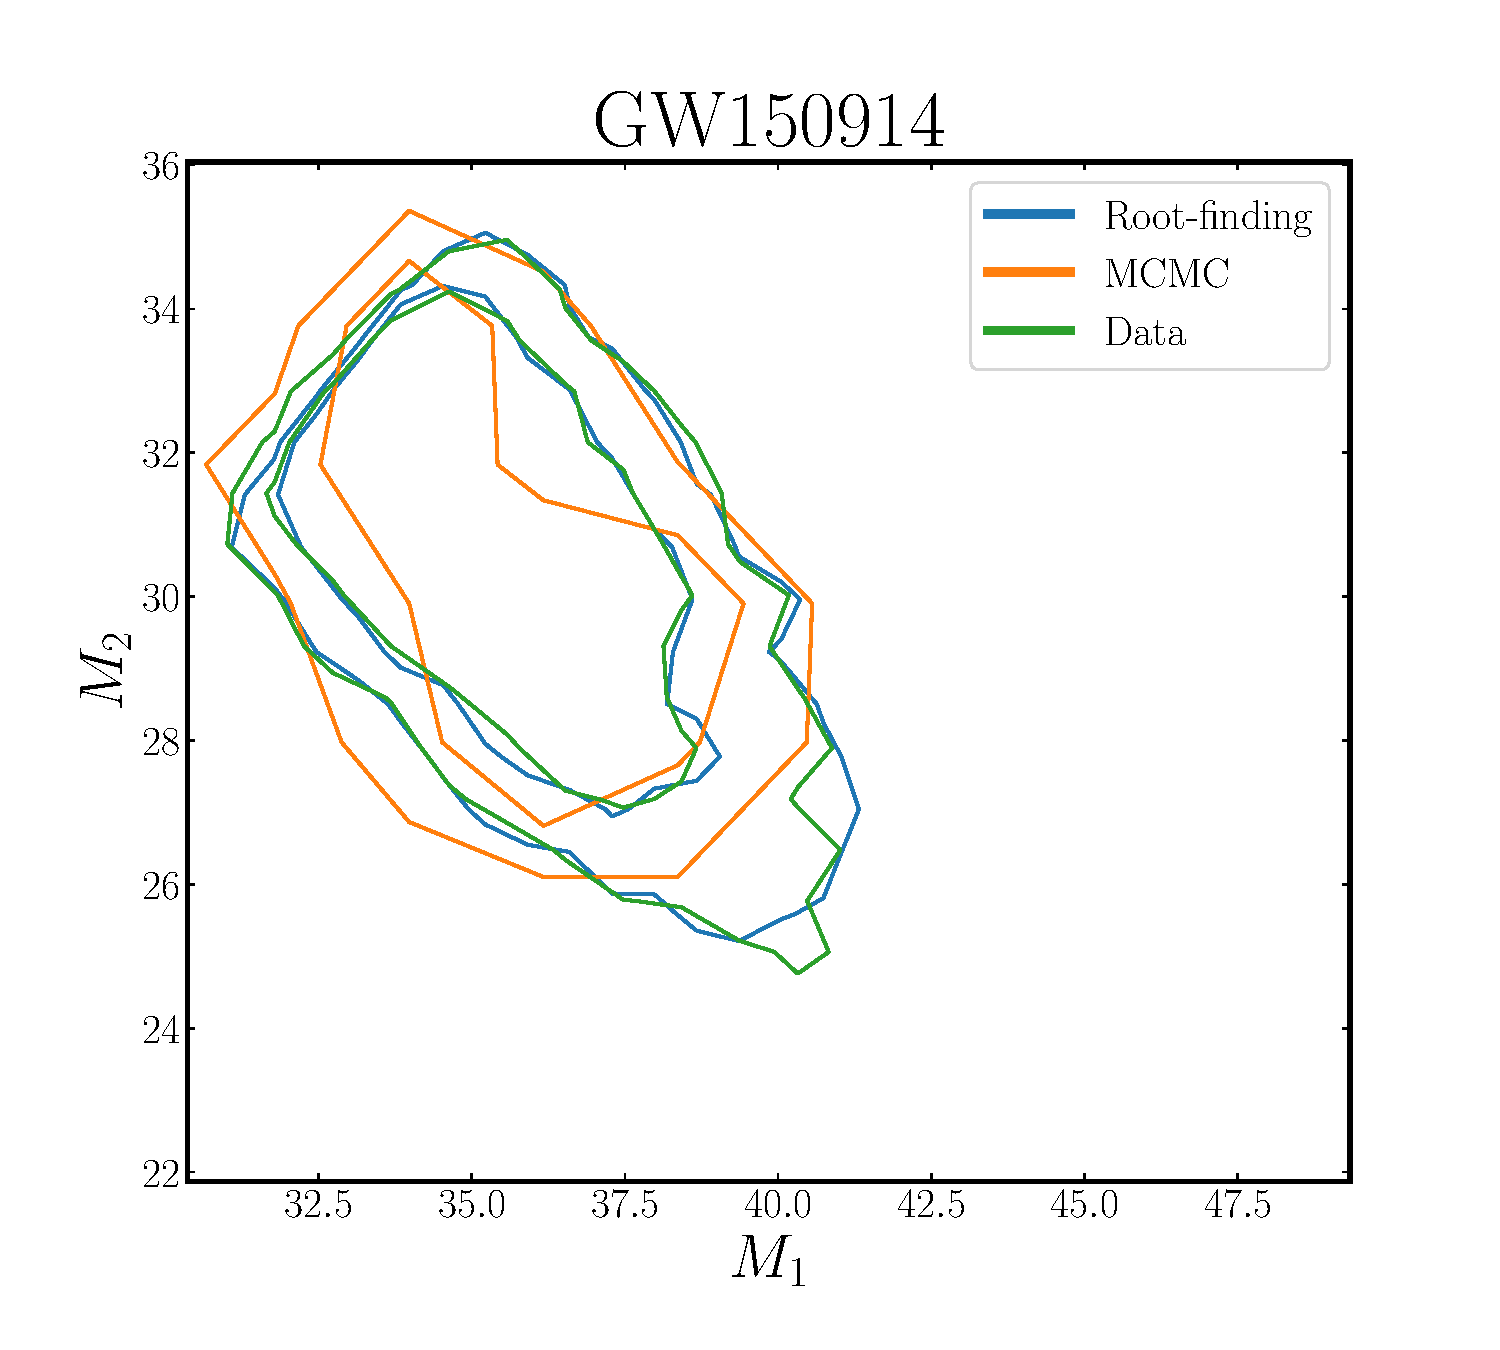
\includegraphics[width=0.49\textwidth]{figures/GW150914_reprojection.pdf}
\caption{Reprojecting the posterior in evolutionary parameter space of GW150914 to observable space.
The blue contour is the reprojected posterior after the root-finding procedure.
The orange contour is the reprojected posterior after the MCMC procedure.
The green contour is the posterior plotted using the original LVK posterior samples.
}
\label{fig:GW150914_reprojection}
\script{figure3_sanityCheck.py}
\end{figure}


% Paragraph discussing the potential application on the population side.
To illustrate the potential benefit of using our method on the population level, we
perform the same analysis for all events in GWTC3. Plotted in figure
\ref{fig:GWTC3_f_acc_mass} is the posterior density in the $m_{1,{\rm
GW}}-f_{\rm acc}$ space for most of the events in GWTC3. Each contour represents
the $68\%$ credible interval of the posterior density for that particular event.
There is a suggestive trend showing that $f_{\rm acc}$ could increase as the mass of
the progenitor increases. Such a trend implies the stable mass transfer 
phase of a less massive binary would be preferentially non-conservative, with
more conservative mass transfer in more massive binary systems.

Note that some events did not pass the KL divergence test we proposed in section
\ref{sec:method}; we do not include these systems in figure
\ref{fig:GWTC3_f_acc_mass}. Binaries that form low-mass compact objects have
lower amounts of fallback and tend to have correspondingly larger variance in
their random natal kicks. Larger kicks can unbind the progenitor binary, or lead
to wide binaries that do not merge within a Hubble time.  In these cases, the
extra variance during the reprojection can produce a posterior that may not
agree with the original posterior, hence yielding a higher KL divergence. 

For high-mass binaries, \texttt{COSMIC} struggles to produce events above the
pair instability supernova mass cutoff $m_{1,{\rm GW}}$, so the posterior in the
evolutionary parameter space only corresponds to part of the posterior in the
observable space below this cutoff, and therefore events beyond the PISN mass
gap also have higher KL divergence. 

Events with more extreme mass ratios are hard to produce with \texttt{COSMIC},
and therefore less likely to be accurately recovered by our method. This could
be due to our method assuming a single value for $f_{\rm acc}$ and $\alpha$ as
discussed in Section~\ref{sec:result}.

Merger observations for which \texttt{COSMIC} struggles are likely to be very
informative about formation channels and binary evolution physics, and are
therefore likely worthy of close study.  We anticipate that future work will
follow up these events in detail.

Figure \ref{fig:GWTC3_f_acc_mass} shows that our method could in principle
reveal the correlation between progenitor parameters and hyperparameters on a
population level. A careful treatment of all events in the catalog and
discussion related to the detailed physical implications of figure
\ref{fig:GWTC3_f_acc_mass} is beyond the scope of this paper.  We defer a
detailed study of the physics related to the population of GW events to future
work. 


\begin{figure}
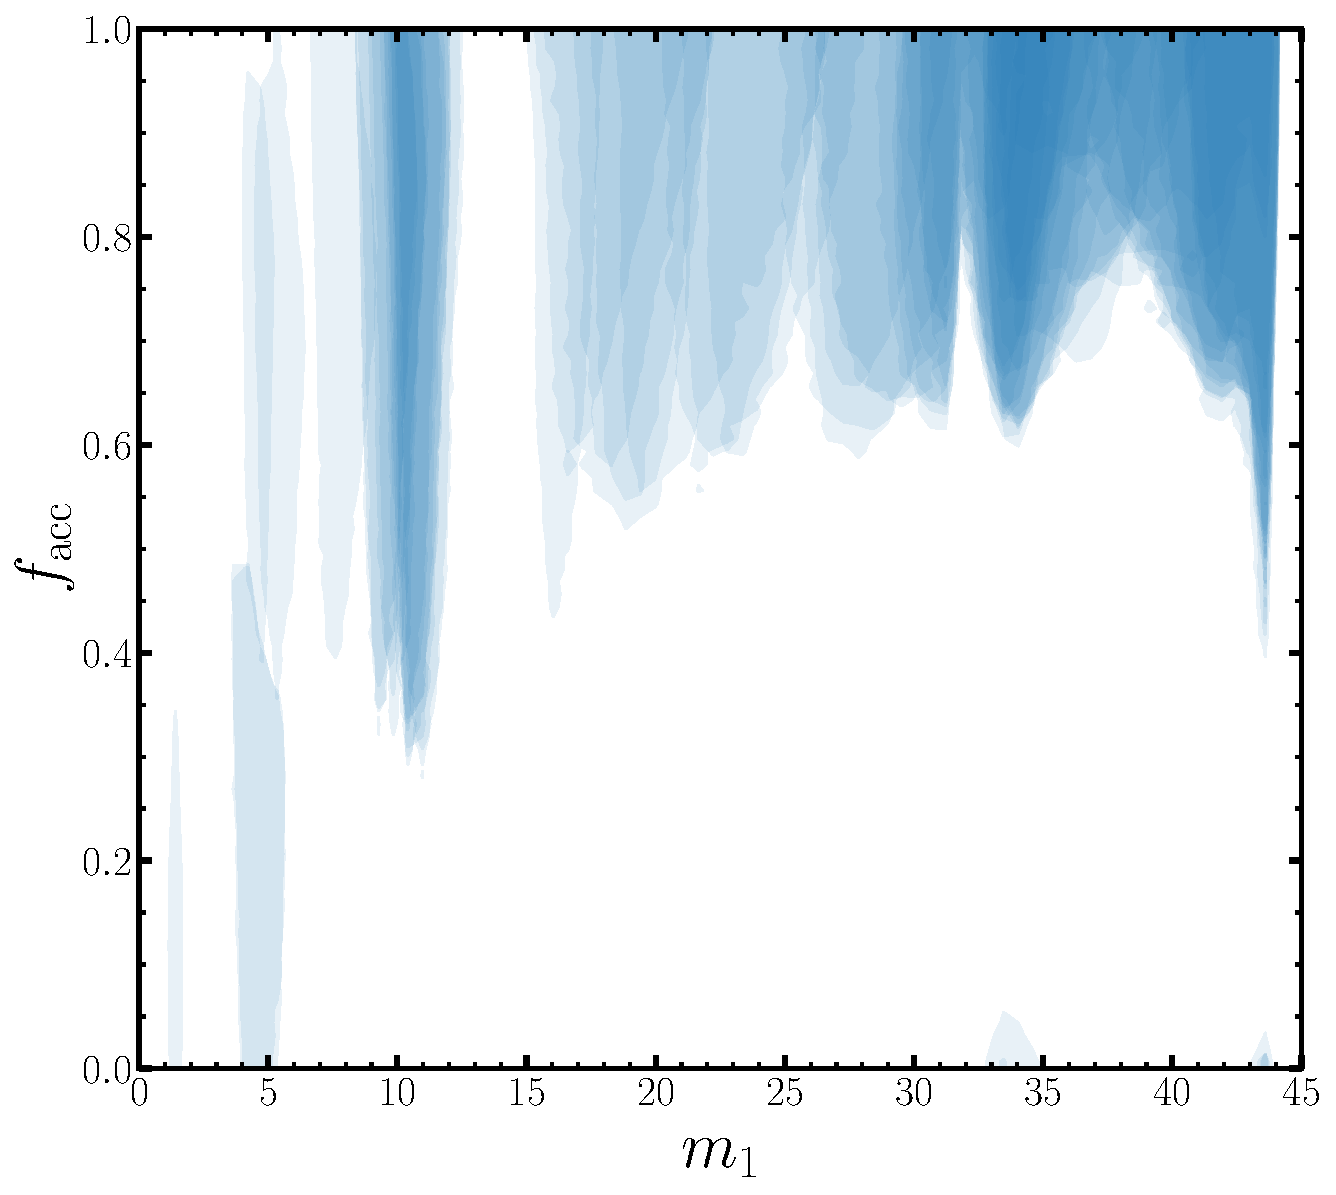
\includegraphics[width=0.49\textwidth]{figures/GWTC3_f_acc_mass.pdf}
\caption{
    The posterior density in the $m_{1,{\rm GW}}-f_{\rm acc}$ space for most of the events in GWTC3.
    Each contour is the $68\%$ credible interval of the posterior density for a particular event. \kw{Check interval number}
    At $m_{1,{\rm GW}} \sim 45 M_{\odot}$, the pair instability supernova mechanism prevents \texttt{COSMIC} from producing events that are more massive than this cutoff.
    Therefore, events with the majority of posterior support above this cutoff is not compatible with \texttt{COSMIC}, hence has a large KL divergence and excluded from this figure.
    On the low mass end, neutron star binaries or neutron star-black hole binaries are subjected to randomness induced by the natal kick,
    also resulting in a larger and fluctuating KL divergence, therefore they are also excluded from the analysis.
}
\label{fig:GWTC3_f_acc_mass}
\script{figure4_population.py}
\end{figure}

\section{Discussion}
\label{sec:discussion}


We present a new pathway to understand binary evolution with GW events in this
paper. Instead of forward modelling an assumed distribution of initial binaries
to the observed population, we find the corresponding evolutionary parameters
event-by-event. In this first work, we showcase the power of the proposed method
with an application to GW150914. We show the joint posterior of the event's
progenitor parameters and hyperparameters.  Our work is both a more efficient
way to study GW event progenitors, and also allows the possibility of
constraining the astrophysics related to binary evolution, especially by
capturing the correlation between hyperparameters in different systems. 

Our results suggest that the accretion efficiency during stable mass transfer
may depend on the primary black hole mass.  In general, our method returns the
joint posterior distribution of progenitor parameters and hyperparameters for
each event, which enables a data-driven way to study the distribution of
hyperparameters.  That is, once we have a catalog of events, each has their own
posterior in the hyperparameter space, and we can employ well-known techniques
such as hierarchical Bayesian analysis to fit a population model to the
distribution of hyperparameters; this avoids making overly-specific assumptions
like fixing the hyperparameters for all types of event. 

% Rate analysis is now just counting, like what's done in phenomenological model, instead of forward modelling.
Working event-by-event as we do permits post-processing application of
 arbitrarily complicated models of star formation and metalliticy evolution by
 re-weighting the samples we obtain \wf{Cite at least Lieke here}. Once we have
 pulled the GW event posterior back from the observable space to the
 evolutionary parameter space, we can apply the same hierarchical inference
 methods currently used to infer the compact binary population to our progenitor
 population.  In particular, we can use our progenitor population to infer the
 formation rate of compact binary population progenitor systems over cosmic time
 without needing to make artifical and simplistic assumptions about the delay
 time distribution or the metallicity-specific star formation rate \wf{again,
 cite Lieke, and also Vitale, Farr, Ng, Rodriguez?}.  Comparing the formation
 rate of progenitors to the star formation rate provides an avenue to check our
 understanding of binary evolution and the relative rate of other formation
 channels.

% Single formation channel and fundamental limitation on that.
While our method allows data-driven exploration of the hyperparameters space for the first time, there are a number of improvements can be implemented in future studies.
In this study we use only \texttt{COSMIC} as our evolutionary function, which by design cannot explain all the events in GWTC3.
For example, event with either of the component mass larger than the PISN gap such as GW190521 cannot be explained by \texttt{COSMIC}.
Alternative channels such as dynamic formation channel will be needed to explain some subset of the events in GWTC3.
As pointed out in the literature \kw{Cite mike}, it is unlikely that all the observed events in GWTC3 can be explained by a single formation channel.
As GW detectors sensitivity increase, we expect to see more and more events that are unusual in some way.
Therefore, having a self-consistence population synthesis code that contains multiple formation channels is essential to accommodate the growing catalog of GW events.
In this paper, our main focus is to illustrate the concept of "back-propagating" GW events posterior sample in this work,
highlighting the capability of our method and motivating the community to build the next generation population synthesis code that can work with our method.
To avoid cluttering of focus, we discuss the physical implication of the result presented in this work under our specific assumption (i.e. using \texttt{COSMIC} as our evolutionary function) in a companion paper.


% Randomness paragraph
Due to the implicit definition of random variables in \texttt{COSMIC}, our evolutionary function is stochastic.
This introduces significant inefficiency in our root-finding and sampling algorithm.
The main stochasticity in \texttt{COSMIC} comes from natal kick, which significantly affect the evolution pathway of low mass events such as BNS events.
The effect of natal kick is suppressed for heavier mass events due to fallback.
This means events with lighter masses are subject to stochasticity of the function,
where the sampling process for heavier events behaves as if the evolutionary function we use are deterministic.
% Indeed, we see this behavior in a couple of case studies.
% For heavy event such as GW150914, the reprojected posterior agrees with the data posterior.
% For light event such as GW170817, although during the root-finding process the convergence criteria is met,
% the reprojected posterior does not agree with the data posterior.
Due to computational limitation, we only try 1000 different initial guesses per posterior sample in the root-finding process.
This means any posterior sample that has a probability of merging rarer than 1 in 1000 could be missed.
Obviously the problems which comes with the randomness can be alleviated by performing more tries per posterior sample,
but this is not scalable in practice.
On top of limitation in efficiency, some formation channels require explicit control of random variables by construction.
For example, in a dynamical formation scenario such as binaries that form in a globular cluster,
each binary has some probability of undergoing a multi-body encounter with another member in the cluster.
These encounter probability distributions are either studied with direct N-body simulations or semi-analytical methods.
In both cases, each member of the cluster is no longer completely independent of the other members, but coupled through the encounter probability distribution.
By studying the encounter probability distribution, we can infer the properties of the environment which the binary lives in.
This can only be done if we have explicit control over the random variables that characterize the encounter probability distribution.

% Need for selection bias to recover intrinsic distribution



% Gradient decending in the evolutionary parameter space is much more efficent than rejection sampling.
% Potential pitfall of interpreting this result.
% Need for full autodiff.

% By leveraging gradient-based optimization strategy, obtaining posterior samples in the evolutionary parameter space is much more efficient than rejection sampling.
% In each optimization step during the root-finding process, the current state of the guess and its gradient provide useful information about where the root might be.
% In contrast to sampling algorithm, which discard the sample whenever it is not accepted.
% This greatly benefit the efficiency of the root-finding process.
% On the other hand, this method is not a sampling algorithm, but a coordinate transform of the posterior samples.
% One should pay extra caution in interpreting the posterior samples in the evolutionary parameter space.
% Since posterior samples in the observable space can in principle have multiple roots in the evolutionary parameter space,
% the relatively weighting of these roots becomes ambiguous when the number of roots is large.
% For example, should we consider roots that are close to each other a single root or multiple roots?
% If we have two clusters of roots, the relative number of roots within each cluster would determine the relative weight of each mode.
% Note that since they both map to the same observable posterior sample within the acceptance threshold, all weighting assigned are equally valid from a "matching data" standpoint.
% This leave the interpretation of the posterior in the evolutionary parameter space ambiguous.
% In our case, we found empirically each posterior sample may at most only correspond to a handful of roots (most of the posterior samples have a unique root.), therefore we choose to assign equal weight to each root.

% The potential reason for the good agreement between MCMC and the root finding is due to the behavior of posterior in the evolutionary parameter space are larger determined by the posterior distribution in the observable space instead of multiple possible roots per posterior sample.
% We have also compared two MCMC results, one is initialized using the roots and another is initialized using samples drawn from a uniform prior.
% We found empirically the MCMC result using the roots as initialization converges at least an order of magnitude faster than the uniform prior initialization.
% This makes sense since the roots basically eliminate the long burn-in needed to go from random location in the evolutionary parameters to the most probable region.
% We leave a detail comparison between this method and direct sampling to future studies.

Another technical note is we use finite differencing to estimate the gradient of the objective function, which could be a significant source of error near transition points in the evolutionary parameter space.
Also, finite differencing is increasing inefficiency as we increase the dimensionality of the problem.
To improve the accuracy and efficiency in estimating the gradient of objective function, automatic differentiation is a promising feature that modeler should consider incorporating in their population synthesis code in the future.


To summarize, we propose a novel method to recover the posterior samples in the evolutionary parameter space for each GW event.
We point out hyperparameters in the usual population synthesis simulation context are not actually parameters related to the population,
but parameters about the evolutionary function.
This means the binary evolution functions can be constrained on an individual event basis.
We "back propagate" the posterior in the observable space to the evolutionary parameter space,
thus allowing us to study hyperparameters and its correlation with progenitor parameters in a data-driven manner.
Our method makes less assumptions than the traditional forward modelling approach,
which often fix the hyperparameters across the entire population.
Since we are not limited to the fixed hyperparameters assumption, we can explore the behavior of the hyperparameters across the population much more efficiently.
While our work lays down a data analysis pathway to understand the population of GW events,
no physics can be learned without a comprehensive physical model.
We hope this letter would motivate the community to build the next generation population synthesis codes that have the following properties:
first, they should have explicit control over the random variables so marginalizing over random variables can be done more precisely;
second, they should be as automatically differentiable as much as possible so exploring the evolutionary parameter space is efficient.
Combining this work and the next generation population synthesis code,
we can explore the full parameter space of binary evolution models with the next-generation GW detectors network in the near future.


\section{Acknowledgement}

\bibliography{bib}

\end{document}
